\chapter{Combinatoire}

\section{Exemples introductifs}

La combinatoire consiste à \emph{compter sans énumérer un à un}. 
Les deux premiers outils sont le \textbf{principe additif} et le 
\textbf{principe multiplicatif}.

\subsection{Les principes additif et multiplicatif}

\paragraph{Principe additif.}
Lorsqu’un choix se fait \emph{dans une catégorie ou dans une autre}, ces catégories n’ayant
aucun choix en commun, on additionne les nombres de choix.

\medskip

\noindent\textbf{Exemple.} À la sortie du lycée, Tiana peut acheter un goûter :
\begin{itemize}
    \item un \emph{koba} parmi \(3\) sortes ;
    \item ou un \emph{mokary} parmi \(2\) sortes.
\end{itemize}
Combien de choix a-t-il ?

\[
3+2=5.
\]

Il y a donc \(\boxed{5}\) choix possibles.

\paragraph{Principe multiplicatif.}
Lorsqu’un choix se fait en plusieurs étapes successives, et que le nombre de possibilités
à chaque étape ne dépend pas des choix déjà faits, on multiplie.

\medskip

\noindent\textbf{Exemple.} Sur son chemin, Tiana peut composer son repas avec :
\begin{itemize}
    \item un plat parmi \(3\) possibilités : \emph{romazava}, \emph{ravitoto}, \emph{vary amin’anana} ;
    \item une boisson parmi \(2\) possibilités : eau ou jus.
\end{itemize}
Le nombre de repas possibles est

\[
3\times 2=6.
\]

Il y a donc \(\boxed{6}\) repas différents.

\medskip

\noindent\textbf{Première généralisation.}
Si une expérience se déroule en \(p\) étapes, et qu’il y a respectivement
\(n_1,n_2,\dots,n_p\) choix à chaque étape, alors le nombre total d’issues est
\[
n_1n_2\cdots n_p.
\]

\subsection{Le principe de l’arbre des choix}

L’arbre des choix permet de visualiser un raisonnement multiplicatif.

\medskip

\noindent\textbf{Exemple : menu malgache.}
On choisit :
\begin{itemize}
    \item une entrée : \emph{sambos} ou \emph{achards} ;
    \item un plat : \emph{romazava} ou \emph{ravitoto} ;
    \item un dessert : \emph{koba} ou \emph{mokary}.
\end{itemize}

Chaque menu correspond à un chemin dans l’arbre ci-dessous.

\begin{center}
\fitfig{%
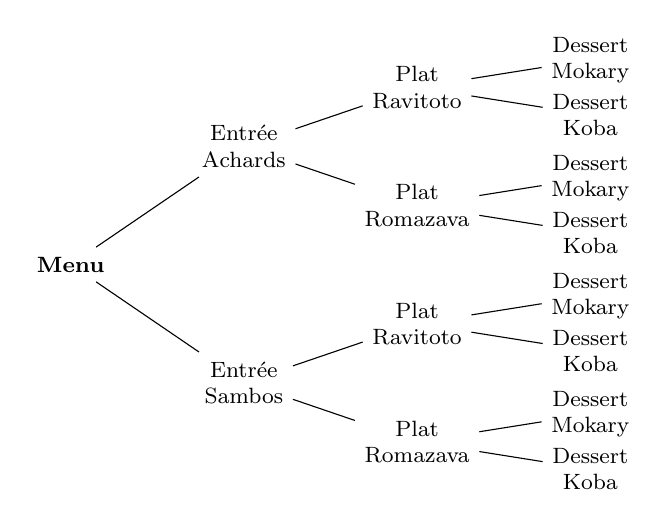
\begin{tikzpicture}[
  grow=right, align=center, font=\footnotesize,
  level 1/.style={sibling distance=30mm,level distance=22mm},
  level 2/.style={sibling distance=15mm,level distance=22mm},
  level 3/.style={sibling distance=7mm,level distance=22mm},
  edge from parent/.style={draw,-}]
\node {\textbf{Menu}}
  child { node {Entrée\\Sambos}
    child { node {Plat\\Romazava} child { node {Dessert\\Koba}} child { node {Dessert\\Mokary}} }
    child { node {Plat\\Ravitoto} child { node {Dessert\\Koba}} child { node {Dessert\\Mokary}} } }
  child { node {Entrée\\Achards}
    child { node {Plat\\Romazava} child { node {Dessert\\Koba}} child { node {Dessert\\Mokary}} }
    child { node {Plat\\Ravitoto} child { node {Dessert\\Koba}} child { node {Dessert\\Mokary}} } };
\end{tikzpicture}}
\end{center}

Comme il y a \(2\) choix pour l’entrée, \(2\) choix pour le plat et \(2\) choix pour le dessert,
on obtient

\[
2\times 2\times 2=8.
\]

Il y a donc \(\boxed{8}\) menus possibles.

\medskip

\noindent
L’arbre sert surtout à \emph{voir} les possibilités ; le calcul se fait ensuite par multiplication.

\subsection{Le principe des codes : avec répétitions et sans répétitions}

\paragraph{Codes avec répétition autorisée.}
On forme un code à \(3\) chiffres avec les symboles
\[
0,\;1,\;2,\;3.
\]
Chaque position peut contenir n’importe lequel des \(4\) symboles.

Le nombre de codes est donc
\[
4\times 4\times 4=4^3=64.
\]

Il y a \(\boxed{64}\) codes possibles.

\medskip

\noindent\textbf{Généralisation.}
Si un code est de longueur \(p\) et si l’on dispose de \(n\) symboles, alors avec répétition autorisée,
le nombre total de codes est
\[
\boxed{n^p}.
\]

\paragraph{Codes sans répétition.}
On reprend les symboles \(0,1,2,3\), mais cette fois un symbole ne peut pas être utilisé deux fois.

\begin{itemize}
    \item \(4\) choix pour le premier chiffre ;
    \item \(3\) choix pour le deuxième ;
    \item \(2\) choix pour le troisième.
\end{itemize}

Donc
\[
4\times 3\times 2=24.
\]

Il y a \(\boxed{24}\) codes possibles.

\medskip

\noindent\textbf{Généralisation.}
Avec \(n\) symboles distincts et un code de longueur \(p\) sans répétition (avec \(p\le n\)), on obtient
\[
\boxed{n(n-1)(n-2)\cdots(n-p+1)}.
\]

Cette quantité apparaîtra plus tard sous le nom d’\emph{arrangement}.

\subsection{Choisir sans ordre et avec ordre}

On termine par une distinction fondamentale : 
\emph{l’ordre compte-t-il ou non ?}

\subsubsection{Choix sans ordre}

\noindent\textbf{Exemple.}
Dans un \emph{fokontany}, \(n\) habitants se portent volontaires pour représenter le quartier.
On veut en choisir \(2\) (avec \(n\ge 2\)), sans attribuer de rôle particulier.

Ici, choisir \(\{A,B\}\) revient au même que choisir \(\{B,A\}\) :
\textbf{l’ordre ne compte pas}.

\medskip

Si l’on comptait avec ordre, on aurait :
\[
n(n-1)
\]
possibilités, car :
\begin{itemize}
    \item \(n\) choix pour la première personne ;
    \item \(n-1\) choix pour la deuxième.
\end{itemize}

Mais chaque paire a été comptée \emph{deux fois} :
\[
(A,B)\quad \text{et}\quad (B,A).
\]
Donc le nombre de choix sans ordre est
\[
\frac{n(n-1)}{2}.
\]

On note ce nombre \(\binom{n}{2}\) (on lit « \(2\) parmi \(n\) ») :
\[
\binom{n}{2}=\frac{n(n-1)}{2}.
\]

\medskip

\noindent\textbf{Exemple numérique.}
S’il y a \(n=5\) volontaires, alors
\[
\binom{5}{2}=\frac{5\times 4}{2}=10.
\]

\subsubsection{Choix avec ordre}

\noindent\textbf{Exemple.}
Parmi \(n\) candidats, on veut choisir
\begin{itemize}
    \item un \emph{sefo fokontany} ;
    \item puis un adjoint, qui est une autre personne.
\end{itemize}

Cette fois, les rôles sont différents :
choisir \(A\) comme sefo et \(B\) comme adjoint
n’est pas la même chose que choisir \(B\) comme sefo et \(A\) comme adjoint.

\medskip

Le nombre de choix est donc
\[
n(n-1).
\]

\noindent\textbf{Exemple numérique.}
Pour \(n=5\) candidats :
\[
5\times 4=20.
\]

Il y a donc \(\boxed{20}\) façons de choisir un sefo fokontany et un adjoint parmi \(5\) personnes.

\subsection{À retenir}

\begin{itemize}
    \item \textbf{Principe additif :} si l’on choisit \emph{ceci ou cela}, sans choix commun aux deux, on additionne.
    \item \textbf{Principe multiplicatif :} si l’on choisit \emph{ceci puis cela}, on multiplie.
    \item \textbf{Arbre des choix :} il permet de visualiser une situation de comptage.
    \item \textbf{Code avec répétition :} avec \(n\) symboles et \(p\) positions, on obtient \(n^p\).
    \item \textbf{Code sans répétition :} avec \(p\le n\), on obtient \(n(n-1)\cdots(n-p+1)\).
    \item \textbf{Choix sans ordre :} pour choisir \(2\) personnes parmi \(n\), on obtient
    \[
    \binom{n}{2}=\frac{n(n-1)}{2}.
    \]
    \item \textbf{Choix avec ordre :} pour deux rôles distincts, on obtient
    \[
    n(n-1).
    \]
\end{itemize}

\section{Factorielle et coefficients binomiaux}

Dans cette section, on passe des exemples concrets aux premières formules générales
de combinatoire.

\subsection{Des choix successifs à la factorielle}

Supposons que \(n\) personnes doivent se placer en file indienne.

\begin{itemize}
    \item Il y a \(n\) choix pour la première place ;
    \item puis \(n-1\) choix pour la deuxième ;
    \item puis \(n-2\) choix pour la troisième ;
    \item etc. ;
    \item enfin \(1\) choix pour la dernière.
\end{itemize}

Le nombre total de files possibles est donc
\[
n(n-1)(n-2)\cdots 2\cdot 1.
\]

\medskip

On introduit alors la notation suivante :

\[
\boxed{n! = n(n-1)(n-2)\cdots 2\cdot 1}
\]

On lit \(n!\) : \emph{\(n\) factorielle}.

\medskip

Par convention, on pose aussi
\[
\boxed{0! = 1.}
\]

Un rangement de \(n\) objets distincts dans un ordre s’appelle une \textbf{permutation}
de ces objets. Il y a donc \(n!\) permutations de \(n\) objets distincts.

\paragraph{Exemple 1.}
Avec \(4\) élèves, le nombre de façons de se ranger est
\[
4! = 4\times 3\times 2\times 1 = 24.
\]

\paragraph{Exemple 2.}
Dans un \emph{fokontany}, \(5\) personnes doivent occuper \(5\) rôles distincts
(sefo, adjoint, secrétaire, trésorier, conseiller).
Le nombre d’affectations possibles est
\[
5! = 120.
\]

\subsection{Schéma d’ensemble}

On peut résumer l’idée générale par le schéma suivant :

\begin{center}
\fbox{
\begin{minipage}{\linewidth}
\[
\resizebox{\linewidth}{!}{$\displaystyle
\boxed{\text{choix successifs}}
\;\Longrightarrow\;
\boxed{n!}
\;\Longrightarrow\;
\boxed{\text{\footnotesize{choix ordonné de} }k\text{\footnotesize{ personnes parmi } }n}
\;\Longrightarrow\;
\boxed{\binom{n}{k}}
$}
\]
\end{minipage}
}
\end{center}

\medskip

Autrement dit :
\begin{itemize}
    \item quand on choisit \emph{successivement} plusieurs personnes, on multiplie ;
    \item quand on choisit \emph{toutes} les \(n\) personnes dans un ordre, on obtient \(n!\) ;
    \item quand on choisit seulement \(k\) personnes dans un ordre, on obtient un produit plus court (voir ci-après) ;
\end{itemize}

\subsection{Choix ordonné de \(k\) personnes parmi \(n\)}

Supposons que \(n\) candidats soient disponibles et que l’on veuille attribuer
\(k\) rôles distincts, avec \(k\le n\) (une même personne n’a qu’un rôle).

\begin{itemize}
    \item \(n\) choix pour le premier rôle ;
    \item \(n-1\) choix pour le deuxième ;
    \item \(n-2\) choix pour le troisième ;
    \item \(\dots\)
    \item \(n-k+1\) choix pour le \(k\)-ième rôle.
\end{itemize}

Le nombre total de choix ordonnés est donc
\[
n(n-1)(n-2)\cdots (n-k+1).
\]

On peut aussi l’écrire avec les factorielles :
\[
\boxed{n(n-1)\cdots(n-k+1)=\frac{n!}{(n-k)!}}
\]

Un tel choix ordonné s’appelle un \textbf{arrangement} de \(k\) objets parmi \(n\) : c’est la
quantité déjà rencontrée avec les codes sans répétition.

\paragraph{Exemple 3.}
Parmi \(10\) habitants, on veut choisir trois personnes différentes :
\begin{itemize}
    \item un président ;
    \item un vice-président ;
    \item un secrétaire.
\end{itemize}

Le nombre de choix est
\[
10\times 9\times 8 = 720.
\]

\medskip

\begin{center}
\begin{minipage}{\linewidth}
\[
\resizebox{\linewidth}{!}{$\displaystyle
\boxed{\text{choix ordonné de }k\text{ personnes parmi }n
= n(n-1)\cdots(n-k+1)=\frac{n!}{(n-k)!}}
$}
\]
\end{minipage}
\end{center}

\subsection{Petit schéma de compréhension}

Voici le raisonnement à retenir :

\begin{center}
\[
\boxed{\text{groupe sans ordre}}
\quad\Longleftarrow\quad
\boxed{\text{groupe avec ordre}}
\quad\text{puis on divise par }k!
\]
\[
\frac{n(n-1)\cdots(n-k+1)}{k!}
=
\binom{n}{k}
\]
\end{center}

Soit \(0\le k\le n\). On note \(\binom{n}{k}\) (on lit « \(k\) parmi \(n\) » ; on trouve aussi
l’écriture \(C(n,k)\)) le nombre de façons de choisir \(k\) personnes parmi \(n\), sans ordre.
Chaque groupe de \(k\) personnes apparaît exactement \(k!\) fois parmi les choix ordonnés
(une fois pour chaque ordre possible de ses membres). Donc
\(k!\binom{n}{k}=\dfrac{n!}{(n-k)!}\), c'est-à-dire
\[
\binom{n}{k}=\frac{n!}{k!\,(n-k)!}.
\]

On peut aussi résumer sous forme de tableau :

\begin{center}
\begin{tabular}{|c|c|c|}
\hline
\textbf{Situation} & \textbf{Ordre ?} & \textbf{Nombre de choix} \\
\hline
Choisir un sefo puis un adjoint & Oui & \(n(n-1)\) \\
\hline
Choisir \(2\) représentants & Non & \(\binom{n}{2}\) \\
\hline
Choisir \(k\) personnes avec rôles distincts & Oui & \(\dfrac{n!}{(n-k)!}\) \\
\hline
Choisir \(k\) personnes sans rôle & Non & \(\binom{n}{k}\) \\
\hline
\end{tabular}
\end{center}

\subsection{Ranger des objets qui se répètent : les anagrammes}

Une \textbf{anagramme} d’un mot est un mot (ayant un sens ou non) écrit avec exactement les
mêmes lettres, chacune autant de fois.

\paragraph{Exemple 4.}
Combien d’anagrammes a le mot TANANA ? Il a \(6\) lettres : trois A, deux N et un T.

On commence par distinguer les lettres identiques en les numérotant :
\(T,\ A_1,\ A_2,\ A_3,\ N_1,\ N_2\). Ce sont \(6\) objets distincts, que l’on peut ranger de
\(6!=720\) façons.

On efface ensuite les numéros. Une anagramme donnée, par exemple ATANAN, provient de
\(3!\) façons de placer \(A_1,A_2,A_3\) aux places des A, et de \(2!\) façons de placer
\(N_1,N_2\) aux places des N, soit \(3!\times 2!=12\) rangements. Le nombre d’anagrammes est donc
\[
\frac{6!}{3!\,2!}=\frac{720}{12}=60.
\]

\paragraph{Cas général.}
On range \(n\) objets formés de \(n_1\) objets identiques d’une première sorte, \(n_2\) objets
identiques d’une deuxième sorte, \dots, \(n_r\) objets identiques d’une \(r\)-ième sorte, avec
\(n_1+n_2+\dots+n_r=n\). Le même raisonnement donne
\[
\boxed{\frac{n!}{n_1!\,n_2!\cdots n_r!}}
\]
rangements. On parle aussi de \textbf{permutations avec répétitions}.

Par exemple, les mots formés de \(k\) chiffres \(1\) et de \(n-k\) chiffres \(0\) sont au nombre
de \(\dfrac{n!}{k!\,(n-k)!}=\binom{n}{k}\). On retrouvera ces mots dans la section sur les bijections.

\subsection{À retenir}

\begin{itemize}
    \item
    \[
    \boxed{n!=n(n-1)(n-2)\cdots 2\cdot 1}
    \]
    compte les façons de ranger \(n\) objets distincts dans un ordre (les permutations).

    \item
    \[
    \boxed{\frac{n!}{(n-k)!}}
    \]
    compte les choix ordonnés de \(k\) objets parmi \(n\) (les arrangements).

    \item
    \[
    \boxed{\binom{n}{k}=\frac{n!}{k!(n-k)!}}
    \]
    compte les choix sans ordre de \(k\) objets parmi \(n\).

    \item En particulier,
    \[
    \boxed{\binom{n}{2}=\frac{n(n-1)}{2}.}
    \]

    \item Pour ranger \(n\) objets répartis en \(r\) sortes, avec \(n_1\), \(n_2\), \dots, \(n_r\)
    objets identiques de chaque sorte (anagrammes) :
    \[
    \boxed{\frac{n!}{n_1!\,n_2!\cdots n_r!}}
    \]
\end{itemize}

\subsection{Exercices}

\paragraph{Exercice 1.}
Lors d’une fête communale, \(n\) personnes sont candidates pour participer à l’organisation.

\begin{enumerate}
    \item Combien y a-t-il de façons de choisir \(4\) personnes (avec \(n\ge 4\)) et de leur attribuer les rôles suivants :
    président, vice-président, secrétaire, trésorier ? (Une même personne n’a qu’un rôle.)

    \item Combien y a-t-il de façons de choisir simplement un groupe de \(4\) personnes, sans rôle ?

    \item Retrouver à partir de la question 1 la formule
    \[
    \binom{n}{4}=\frac{n!}{4!(n-4)!}.
    \]

    \item Calculer \(\binom{11}{4}\).

    \item Combien y a-t-il de façons de choisir \(4\) personnes parmi \(11\), dont un président et un
    secrétaire (deux rôles distincts), les deux autres membres n’ayant pas de rôle particulier ?
\end{enumerate}

\paragraph{Exercice 2 --- Défi des fokontany.}
Trois fokontany, appelés \(A\), \(B\) et \(C\), présentent chacun \(4\) candidats
pour organiser une fête communale. Il y a donc \(12\) candidats au total.

On souhaite former un comité de \(5\) personnes.

\begin{enumerate}
    \item Combien de comités de \(5\) personnes peut-on former sans aucune contrainte ?

    \item On exige désormais que chacun des trois fokontany soit représenté
    par au moins une personne.
    
    Combien de comités peut-on former ?
    
    \emph{Indication :} compter tous les comités, puis retirer ceux dans lesquels
    l'un des fokontany n'est pas représenté.

    \item Dans chaque comité satisfaisant la condition précédente, on désigne :
    \begin{itemize}
        \item un président ;
        \item un trésorier.
    \end{itemize}
    
    Le président et le trésorier doivent appartenir à deux fokontany différents.
    Une organisation est un comité muni de son président et de son trésorier.
    
    Combien d'organisations différentes peut-on former ?

    \emph{Indication :} on pourra commencer par choisir les fokontany du président
    et du trésorier, puis les personnes occupant ces fonctions, et enfin les trois
    autres membres du comité.

    \item Soa et Tovo sont deux candidats du fokontany \(A\). À la suite d'un
    désaccord, ils refusent de siéger ensemble dans le même comité.
    
    Combien de comités de \(5\) personnes peut-on former si :
    \begin{itemize}
        \item chacun des trois fokontany doit être représenté ;
        \item Soa et Tovo ne peuvent pas appartenir simultanément au comité ?
    \end{itemize}

    \item On impose maintenant simultanément toutes les contraintes suivantes :
    \begin{itemize}
        \item le comité contient \(5\) personnes ;
        \item chacun des trois fokontany est représenté ;
        \item le président et le trésorier appartiennent à deux fokontany différents ;
        \item Soa et Tovo ne siègent pas ensemble.
    \end{itemize}
    
    Combien d'organisations différentes peut-on former ?

    \emph{Indication :} partir du résultat de la question 3 et retirer les
    organisations interdites contenant à la fois Soa et Tovo. Pour compter ces
    organisations interdites, distinguer plusieurs cas selon les fonctions
    éventuellement occupées par Soa et Tovo.

\end{enumerate}

\noindent
\fbox{\(Q_1=792\)}
\quad
\fbox{\(Q_2=624\)}
\quad
\fbox{\(Q_3=9\,600\)}
\quad
\fbox{\(Q_4=544\)}
\quad
\fbox{\(Q_5=8\,384\)}


\section{Inclusion--Exclusion}

Dans plusieurs problèmes de combinatoire, il est plus simple de compter d'abord
\emph{tous les cas}, puis de retirer les cas interdits.

\[
\boxed{
\text{Nombre de cas valides}
=
\text{Nombre total de cas}
-
\text{Nombre de cas interdits}
}
\]

Cependant, lorsque plusieurs catégories de cas interdits se recouvrent,
certains objets peuvent être retirés plusieurs fois. Il faut alors les ajouter
de nouveau. C'est le principe d'\textbf{inclusion--exclusion}.

\subsection{Deux ensembles}

Soient \(A\) et \(B\) deux ensembles.

Si l'on additionne \(|A|\) et \(|B|\), les éléments appartenant à la fois à
\(A\) et à \(B\) sont comptés deux fois.

Il faut donc retrancher une fois leur intersection :

\[
\boxed{
|A\cup B|
=
|A|+|B|-|A\cap B|
}
\]

\begin{center}
\fitfig{%
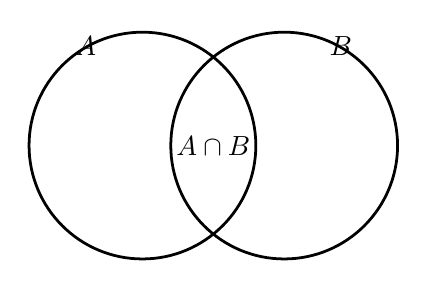
\begin{tikzpicture}[x=0.9cm,y=0.9cm,line width=1pt]
    \draw (-1,0) circle (1.6);
    \draw (1,0) circle (1.6);
    \node at (-1.8,1.4) {\(A\)};
    \node at (1.8,1.4) {\(B\)};
    \node at (0,0) {\(A\cap B\)};
\end{tikzpicture}}
\end{center}

\paragraph{Exemple 1.}
Dans un lycée, \(28\) élèves pratiquent le football, \(19\) pratiquent le
basket-ball et \(8\) pratiquent les deux sports.

Le nombre d'élèves pratiquant au moins l'un des deux sports est

\[
28+19-8=39.
\]

Ainsi,

\[
\boxed{39\text{ élèves pratiquent au moins un des deux sports}.}
\]

\medskip

Sans le terme \(-8\), les \(8\) élèves pratiquant les deux sports seraient
comptés deux fois.

\subsection{Compter par le complémentaire}

Soit \(E\) l'ensemble de toutes les possibilités, et soit \(A\) l'ensemble des
cas interdits.

Alors

\[
\boxed{
|E\setminus A|
=
|E|-|A|
}
\]

\paragraph{Exemple 2.}
On forme un code de \(4\) chiffres à l'aide des chiffres
\[
0,1,2,\dots,9.
\]

Il y a au total

\[
10^4
\]

codes.

Les codes ne contenant aucun \(7\) sont au nombre de

\[
9^4.
\]

Le nombre de codes contenant au moins un \(7\) est donc

\[
\boxed{10^4-9^4=3439.}
\]

\subsection{Retour aux trois fokontany}

Trois fokontany \(A\), \(B\) et \(C\) présentent chacun \(4\) candidats.
On veut former un comité de \(5\) personnes dans lequel chaque fokontany est
représenté.

Il y a au total

\[
\binom{12}{5}
\]

comités.

Notons, pour les comités de \(5\) personnes :
\begin{itemize}
    \item \(E_A\) : les comités ne contenant personne du fokontany \(A\) ;
    \item \(E_B\) : les comités ne contenant personne du fokontany \(B\) ;
    \item \(E_C\) : les comités ne contenant personne du fokontany \(C\).
\end{itemize}

Pour chacun de ces ensembles, on choisit les \(5\) membres parmi les \(8\)
candidats des deux autres fokontany :

\[
|E_A|=|E_B|=|E_C|=\binom{8}{5}.
\]

Il est impossible que deux fokontany soient simultanément absents, car il
faudrait choisir \(5\) personnes parmi les \(4\) candidats du fokontany restant.

Ainsi,

\[
|E_A\cap E_B|
=
|E_A\cap E_C|
=
|E_B\cap E_C|
=
0.
\]

Le nombre de comités valides est donc

\[
\boxed{
\binom{12}{5}
-
3\binom{8}{5}
=
624.
}
\]

Il s'agit déjà d'une application du principe d'inclusion--exclusion.

\subsection{Trois ensembles}

Pour trois ensembles \(A\), \(B\) et \(C\), on commence par additionner leurs
tailles :

\[
|A|+|B|+|C|.
\]

Tout élément appartenant exactement à deux ensembles a été compté deux fois. Un élément appartenant aux trois ensembles a été compté trois fois.
On retranche donc une fois chaque intersection de deux ensembles :

\[
|A|+|B|+|C|-|A\cap B|-|A\cap C|-|B\cap C|.
\]

Mais les éléments de \(A\cap B\cap C\) ont alors été :
\begin{itemize}
    \item comptés trois fois au début ;
    \item puis retranchés trois fois.
\end{itemize}

Ils ne sont donc plus comptés du tout. Il faut les ajouter une fois.

On obtient :

\[
\boxed{
\begin{aligned}
|A\cup B\cup C|
={}&|A|+|B|+|C|\\
&-|A\cap B|-|A\cap C|-|B\cap C|\\
&+|A\cap B\cap C|.
\end{aligned}
}
\]

Les signes alternent donc :

\[
\resizebox{\linewidth}{!}{$\displaystyle
\boxed{
+\text{ ensembles seuls}
\quad
-\text{ intersections de deux ensembles}
\quad
+\text{ intersection des trois ensembles}.
}
$}
\]

\subsection{Forme complémentaire}

Si \(E\) est l'ensemble de toutes les possibilités et si \(A\), \(B\), \(C\)
désignent trois catégories de cas interdits, alors le nombre de cas valides est

\[
|E\setminus(A\cup B\cup C)|.
\]

Par inclusion--exclusion,

\[
\boxed{
\begin{aligned}
|E\setminus(A\cup B\cup C)|
={}&|E|-|A|-|B|-|C|\\
&+|A\cap B|+|A\cap C|+|B\cap C|\\
&-|A\cap B\cap C|.
\end{aligned}
}
\]

\subsection{Exemple numérique}

Parmi les entiers de \(1\) à \(100\), combien sont divisibles par \(2\) ou par
\(5\) ?

Notons :
\[
A=\{\text{multiples de }2\},
\qquad
B=\{\text{multiples de }5\}.
\]

On a

\[
|A|=50,
\qquad
|B|=20.
\]

Les nombres divisibles à la fois par \(2\) et par \(5\) sont les multiples de
\(10\) :

\[
|A\cap B|=10.
\]

Ainsi,

\[
|A\cup B|
=
50+20-10
=
60.
\]

Donc

\[
\boxed{60\text{ entiers sont divisibles par }2\text{ ou par }5.}
\]

Le nombre d'entiers qui ne sont divisibles ni par \(2\), ni par \(5\), est

\[
100-60=40.
\]

\subsection{À retenir}

\begin{center}
\fbox{
\begin{minipage}{0.88\linewidth}
\[
\boxed{
\text{On additionne les cas simples,}
}
\]

\[
\boxed{
\text{on retranche les doubles intersections,}
}
\]

\[
\boxed{
\text{on ajoute les triples intersections, etc.}
}
\]
\end{minipage}
}
\end{center}

Le principe général repose sur une alternance de signes :

\[
\boxed{
+\quad -\quad +\quad -\quad \cdots
}
\]

\subsection{Exercice de compréhension}

Dans une classe de \(40\) élèves :
\begin{itemize}
    \item \(25\) élèves parlent malgache ;
    \item \(18\) élèves parlent français ;
    \item \(10\) élèves parlent les deux langues.
\end{itemize}

\begin{enumerate}
    \item Combien d'élèves parlent au moins l'une des deux langues ?
    \item Combien d'élèves ne parlent aucune de ces deux langues ?
\end{enumerate}

\subsection{Exercice \(+\)}

Parmi les entiers de \(1\) à \(200\), déterminer :
\begin{enumerate}
    \item le nombre d'entiers divisibles par \(3\) ;
    \item le nombre d'entiers divisibles par \(5\) ;
    \item le nombre d'entiers divisibles par \(3\) et par \(5\) ;
    \item le nombre d'entiers divisibles par \(3\) ou par \(5\) ;
    \item le nombre d'entiers divisibles ni par \(3\), ni par \(5\).
\end{enumerate}

\subsection{Exercice \(++\)}

Quatre fokontany présentent chacun \(4\) candidats. On souhaite former un comité
de \(6\) personnes dans lequel chacun des quatre fokontany est représenté.

\begin{enumerate}
    \item Combien de comités de \(6\) personnes peut-on former, sans tenir compte de la condition de
    représentation des fokontany ?

    \item Pour un fokontany fixé, combien de comités ne contiennent aucun de ses
    candidats ?

    \item Pour deux fokontany fixés, combien de comités ne contiennent aucun
    candidat de ces deux fokontany ? Et pour trois fokontany fixés ?

    \item Montrer que le nombre de comités dans lesquels chacun des quatre
    fokontany est représenté est
    \[
    \binom{16}{6}
    -
    4\binom{12}{6}
    +
    \binom{4}{2}\binom{8}{6}.
    \]
    (Les comités sans candidat de trois fokontany donnent \(\binom{4}{6}=0\), donc les termes suivants de
    la formule d’inclusion--exclusion sont nuls.)

\end{enumerate}

\section{Concept : les bijections}

Une méthode fondamentale en combinatoire consiste à remplacer les objets
que l'on souhaite compter par d'autres objets, plus simples à dénombrer.

\subsection{Exemple introductif : Soa, Tovo, Fara, Hery et les mots binaires}

On considère l'ensemble de quatre élèves

\[
E=\{\text{Soa},\text{Tovo},\text{Fara},\text{Hery}\}.
\]

On souhaite former un comité en choisissant certains de ces élèves.
Le comité peut éventuellement être vide.

On fixe l'ordre suivant :

\[
(\text{Soa},\text{Tovo},\text{Fara},\text{Hery}).
\]

À chaque comité, on associe un mot de quatre chiffres composé de \(0\) et de
\(1\) :

\begin{itemize}
    \item on écrit \(1\) lorsque l'élève appartient au comité ;
    \item on écrit \(0\) lorsque l'élève n'appartient pas au comité.
\end{itemize}

Par exemple,

\[
\{\text{Soa},\text{Fara}\}
\longleftrightarrow
1010.
\]

\begin{center}
\fitfig{%
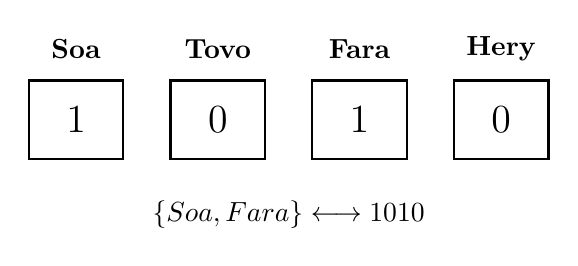
\begin{tikzpicture}[x=1cm,y=1cm,line width=0.8pt]
    \node at (0.75,1.8){\textbf{Soa}};
    \node at (2.55,1.8){\textbf{Tovo}};
    \node at (4.35,1.8){\textbf{Fara}};
    \node at (6.15,1.8){\textbf{Hery}};
    \draw (0.15,0.4) rectangle (1.35,1.4);
    \draw (1.95,0.4) rectangle (3.15,1.4);
    \draw (3.75,0.4) rectangle (4.95,1.4);
    \draw (5.55,0.4) rectangle (6.75,1.4);
    \node at (0.75,0.9){\Large \(1\)};
    \node at (2.55,0.9){\Large \(0\)};
    \node at (4.35,0.9){\Large \(1\)};
    \node at (6.15,0.9){\Large \(0\)};
    \node at (3.45,-0.3){\(\{\text{Soa},\text{Fara}\}\longleftrightarrow 1010\)};
\end{tikzpicture}}
\end{center}

De même,

\[
\{\text{Tovo},\text{Fara},\text{Hery}\}
\longleftrightarrow
0111,
\]

\[
\varnothing
\longleftrightarrow
0000,
\]

et

\[
E
\longleftrightarrow
1111.
\]

Chaque comité donne un unique mot binaire, et chaque mot binaire détermine
un unique comité.

Comme chacune des quatre positions possède deux possibilités, \(0\) ou \(1\),
le nombre de mots binaires est

\[
2\times2\times2\times2=2^4=16.
\]

Il existe donc également \(16\) comités possibles.

Plus généralement, pour un ensemble de \(n\) personnes, chaque sous-ensemble
correspond à un mot binaire de longueur \(n\). Par conséquent,

\[
\boxed{
\text{Un ensemble à \(n\) éléments possède \(2^n\) sous-ensembles.}
}
\]

\subsection{Le concept : une correspondance un-à-un pour compter}

Une \textbf{bijection} entre deux ensembles \(\mathcal A\) et \(\mathcal B\)
est une correspondance telle que :

\begin{itemize}
    \item chaque élément de \(\mathcal A\) correspond à un unique élément de
    \(\mathcal B\) ;
    \item chaque élément de \(\mathcal B\) correspond à un unique élément de
    \(\mathcal A\).
\end{itemize}

Il s'agit donc d'une correspondance parfaite, \emph{un objet contre un objet}.

\begin{center}
\fitfig{%
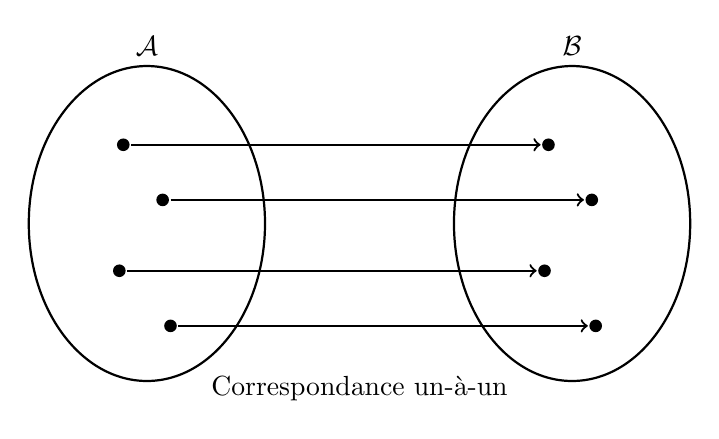
\begin{tikzpicture}[x=1cm,y=1cm,line width=0.8pt]
    \draw (1.7,2) ellipse (1.5 and 2);
    \draw (7.1,2) ellipse (1.5 and 2);
    \node at (1.7,4.25){\(\mathcal A\)};
    \node at (7.1,4.25){\(\mathcal B\)};
    \fill (1.4,3) circle (0.08);
    \fill (1.9,2.3) circle (0.08);
    \fill (1.35,1.4) circle (0.08);
    \fill (2,0.7) circle (0.08);
    \fill (6.8,3) circle (0.08);
    \fill (7.35,2.3) circle (0.08);
    \fill (6.75,1.4) circle (0.08);
    \fill (7.4,0.7) circle (0.08);
    \draw[->] (1.5,3)--(6.7,3);
    \draw[->] (2,2.3)--(7.25,2.3);
    \draw[->] (1.45,1.4)--(6.65,1.4);
    \draw[->] (2.1,0.7)--(7.3,0.7);
    \node at (4.4,-0.1){Correspondance un-à-un};
\end{tikzpicture}}
\end{center}

Lorsqu'il existe une bijection entre deux ensembles finis, ces deux ensembles
ont le même nombre d'éléments :

\[
\boxed{
\mathcal A\longleftrightarrow\mathcal B
\qquad\Longrightarrow\qquad
|\mathcal A|=|\mathcal B|.
}
\]

La stratégie de comptage est donc la suivante :

\begin{center}
\fbox{
\begin{minipage}{0.88\linewidth}
\begin{center}
Pour compter une famille d'objets compliqués, on construit une bijection avec
une famille d'objets plus faciles à compter.
\end{center}

\[
\boxed{
\text{objets compliqués}
\longleftrightarrow
\text{objets simples}
}
\]
\end{minipage}
}
\end{center}

Dans l'exemple précédent,

\[
\boxed{
\text{comités formés parmi \(n\) personnes}
\longleftrightarrow
\text{mots binaires de longueur \(n\)}.
}
\]

\subsection{Exercices}

\subsubsection{Un premier exercice simple}

On considère \(7\) candidats d'un fokontany :

\[
\mathcal{E}=\{A,B,C,D,E,F,G\}.
\]

On souhaite former un comité d'exactement \(3\) personnes.

À chaque comité, on associe un mot binaire de longueur \(7\), dans lequel
\(1\) signifie que le candidat est choisi et \(0\) qu'il ne l'est pas.

Par exemple,

\[
\{A,D,G\}
\longleftrightarrow
1001001.
\]

\begin{enumerate}
    \item Quel comité correspond au mot
    \[
    0110100?
    \]

    \item Quel mot correspond au comité
    \[
    \{B,E,F\}?
    \]

    \item Combien de chiffres \(1\) possède le mot associé à un comité de
    \(3\) personnes ?

    \item Montrer que les comités de \(3\) personnes sont en bijection avec
    les mots binaires de longueur \(7\) contenant exactement \(3\) chiffres
    égaux à \(1\).

    \item En déduire que le nombre de comités est
    \[
    \binom{7}{3}.
    \]

    \item Généraliser : avec \(n\) candidats, combien existe-t-il de comités
    de \(k\) personnes ?
\end{enumerate}

\subsubsection{Chemins sur un quadrillage et coefficient binomial
\(\binom{p+q}{p}\)}

On considère un quadrillage. Pour aller du point \(A\) au point \(B\) par un
chemin de longueur minimale, on est uniquement autorisé à effectuer :

\begin{itemize}
    \item un déplacement vers la droite, noté \(D\) ;
    \item un déplacement vers le haut, noté \(H\).
\end{itemize}

Ici, \(A\) est le coin inférieur gauche et \(B\) le coin supérieur droit d'un quadrillage de
\(4\) carreaux de large et \(3\) de haut. Voici un exemple de chemin comportant \(4\)
déplacements vers la droite et \(3\) déplacements vers le haut.

\begin{center}
\fitfig{%
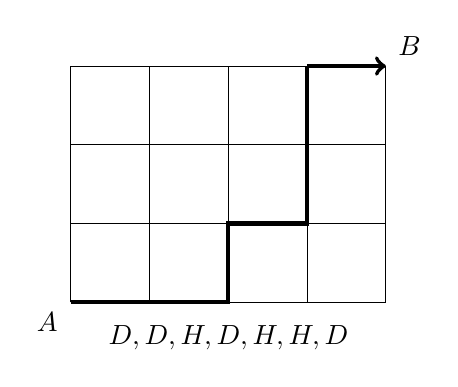
\begin{tikzpicture}[x=1cm,y=1cm]
    \draw[line width=0.3pt,step=1] (0,0) grid (4,3);
    \draw[line width=1.5pt] (0,0)--(1,0)--(2,0)--(2,1)--(3,1)--(3,2)--(3,3);
    \draw[line width=1.5pt,->] (3,3)--(4,3);
    \node at (-0.3,-0.25){\(A\)};
    \node at (4.3,3.25){\(B\)};
    \node at (2,-0.45){\(D,D,H,D,H,H,D\)};
\end{tikzpicture}}
\end{center}

À chaque chemin, on associe le mot formé par la suite de ses déplacements.

Dans l'exemple représenté,

\[
\text{chemin}
\longleftrightarrow
DDHDHHD.
\]

\begin{enumerate}
    \item Combien de lettres \(D\) et de lettres \(H\) possède le mot associé
    au chemin représenté ?

    \item Montrer qu'un chemin minimal de \(A\) vers \(B\) correspond à un
    unique mot contenant \(4\) lettres \(D\) et \(3\) lettres \(H\).

    \item Réciproquement, montrer que tout mot contenant \(4\) lettres \(D\)
    et \(3\) lettres \(H\) définit un unique chemin minimal.

    \item En déduire que le nombre de chemins représentés sur cette grille est
    \[
    \binom{7}{4}
    =
    \binom{7}{3}.
    \]

    \item On considère maintenant un quadrillage nécessitant \(p\) déplacements
    vers la droite et \(q\) déplacements vers le haut. Montrer que les chemins
    minimaux sont en bijection avec les mots de longueur \(p+q\) contenant
    exactement \(p\) lettres \(D\).

    \item En déduire que le nombre de chemins minimaux est
    \[
    \boxed{
    \binom{p+q}{p}
    =
    \binom{p+q}{q}.
    }
    \]
\end{enumerate}

\subsubsection{Partitionner \(2n\) personnes en \(n\) binômes}

On considère \(2n\) personnes distinctes. On souhaite les répartir en
\(n\) binômes, sans distinguer :

\begin{itemize}
    \item l'ordre des deux personnes à l'intérieur d'un binôme ;
    \item l'ordre dans lequel les binômes sont présentés.
\end{itemize}

Par exemple, avec six personnes,

\[
\{\text{Soa},\text{Tovo},\text{Fara},\text{Hery},\text{Mamy},\text{Voara}\},
\]

une partition possible est

\[
\bigl\{
\{\text{Soa},\text{Tovo}\},
\{\text{Fara},\text{Hery}\},
\{\text{Mamy},\text{Voara}\}
\bigr\}.
\]

\begin{center}
\fitfig{%
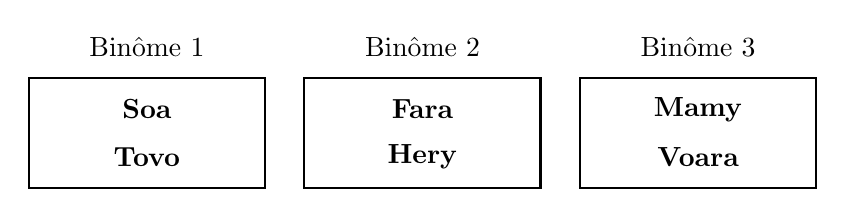
\begin{tikzpicture}[x=1cm,y=1cm,line width=0.8pt]
    \draw (0,0) rectangle (3,1.4);
    \draw (3.5,0) rectangle (6.5,1.4);
    \draw (7,0) rectangle (10,1.4);
    \node at (1.5,1){\textbf{Soa}};
    \node at (1.5,0.4){\textbf{Tovo}};
    \node at (5,1){\textbf{Fara}};
    \node at (5,0.4){\textbf{Hery}};
    \node at (8.5,1){\textbf{Mamy}};
    \node at (8.5,0.4){\textbf{Voara}};
    \node at (1.5,1.8){Binôme \(1\)};
    \node at (5,1.8){Binôme \(2\)};
    \node at (8.5,1.8){Binôme \(3\)};
\end{tikzpicture}}
\end{center}

On numérote maintenant les personnes de \(1\) à \(2n\).

\begin{enumerate}
    \item Pour \(n=2\), écrire toutes les façons de partager les quatre
    personnes
    \[
    \{1,2,3,4\}
    \]
    en deux binômes.

    \item Pour \(n=3\), construire quelques partitions des six personnes
    \[
    \{1,2,3,4,5,6\}
    \]
    en trois binômes.

    \item À une permutation
    \[
    (a_1,a_2,\dots,a_{2n}),
    \]
    on associe les binômes consécutifs
    \[
    \{a_1,a_2\},
    \{a_3,a_4\},
    \dots,
    \{a_{2n-1},a_{2n}\}.
    \]

    Expliquer pourquoi cette correspondance n'est pas encore une bijection.

    \item Pour une partition fixée, expliquer pourquoi on peut :
    \begin{itemize}
        \item échanger les deux personnes dans chacun des \(n\) binômes de
        \(2^n\) façons ;
        \item permuter les \(n\) binômes de \(n!\) façons.
    \end{itemize}

    \item En déduire qu'une même partition est représentée par exactement
    \[
    2^n n!
    \]
    permutations.

    \item Comme il existe \((2n)!\) permutations des \(2n\) personnes,
    montrer que le nombre de partitions en \(n\) binômes est
    \[
    \boxed{
    \frac{(2n)!}{2^n n!}.
    }
    \]

    \item Vérifier que, pour six personnes, le nombre de partitions en trois
    binômes est
    \[
    \frac{6!}{2^3\,3!}=15.
    \]

    \item On appelle \(P_n\) le nombre de partitions de \(2n\) personnes en
    \(n\) binômes. Montrer également que, pour \(n\ge 2\),
    \[
    P_n=(2n-1)P_{n-1}.
    \]

    \item Expliquer cette dernière formule en choisissant d'abord le partenaire
    de la personne numéro \(1\).
\end{enumerate}

\subsection{À retenir}

\begin{center}
\fbox{
\begin{minipage}{0.9\linewidth}
Une bijection permet de compter une famille d'objets en la mettant en
correspondance parfaite avec une autre famille dont le nombre d'éléments est
déjà connu ou plus facile à déterminer.

\[
\boxed{
\mathcal A\longleftrightarrow\mathcal B
\quad\Longrightarrow\quad
|\mathcal A|=|\mathcal B|
}
\]
\end{minipage}
}
\end{center}


